\documentclass[11pt]{article}
\usepackage[utf8]{inputenc}
\usepackage{geometry}
\geometry{a4paper, margin=1in}
\usepackage{hyperref}
\usepackage{graphicx}
\usepackage{tabularx}
\usepackage{booktabs}
\usepackage{enumitem}
\usepackage{amsmath}
\usepackage{amssymb}
\usepackage{xcolor}
\usepackage{tikz}
\usetikzlibrary{shapes,arrows.meta,positioning,calc}

\title{Evaluation Metrics --- A Complete Guide \\ \large Landslide Identification Using Machine Learning}
\author{}
\date{2026-03-17}

\begin{document}

\maketitle

\noindent This document explains every evaluation metric used in this project with simple language, formulas, and worked numerical examples.
Throughout, we use a small toy scenario (10 satellite images) so you can follow the arithmetic by hand, then relate each metric to the real project results.

% ============================================================================
\section{The Toy Dataset: 10 Satellite Images}
% ============================================================================

Suppose our model evaluates 10 satellite images.
The \textbf{actual truth} and the \textbf{model's prediction} are shown below:

\begin{center}
\renewcommand{\arraystretch}{1.15}
\begin{tabular}{cccc}
\toprule
\textbf{Image} & \textbf{Actual} & \textbf{Predicted} & \textbf{Correct?} \\ \midrule
1  & Landslide       & Landslide        & \checkmark \\
2  & Landslide       & Landslide        & \checkmark \\
3  & Landslide       & No Landslide     & $\times$ \\
4  & Landslide       & Landslide        & \checkmark \\
5  & No Landslide    & Landslide        & $\times$ \\
6  & No Landslide    & No Landslide     & \checkmark \\
7  & No Landslide    & No Landslide     & \checkmark \\
8  & No Landslide    & No Landslide     & \checkmark \\
9  & No Landslide    & No Landslide     & \checkmark \\
10 & No Landslide    & No Landslide     & \checkmark \\
\bottomrule
\end{tabular}
\end{center}

\noindent From this table we can count four fundamental quantities:

\begin{center}
\renewcommand{\arraystretch}{1.3}
\begin{tabular}{lcp{7.5cm}}
\toprule
\textbf{Name} & \textbf{Count} & \textbf{Meaning} \\
\midrule
True Positive (TP)  & 3 & Model said \textit{Landslide} and it \textbf{was} a landslide (images 1, 2, 4) \\
False Positive (FP) & 1 & Model said \textit{Landslide} but it was \textbf{not} (image 5) \\
False Negative (FN) & 1 & Model said \textit{No Landslide} but it \textbf{was} one (image 3) \\
True Negative (TN)  & 5 & Model said \textit{No Landslide} and it was \textbf{correct} (images 6--10) \\
\bottomrule
\end{tabular}
\end{center}

\noindent These four numbers are the building blocks for every metric below.

% ============================================================================
\section{Confusion Matrix}
% ============================================================================

A \textbf{Confusion Matrix} arranges TP, FP, FN, and TN into a table so you can see at a glance \emph{where} the model gets confused.

\subsection{Binary Example (2 classes)}

\begin{center}
\begin{tabular}{l|cc}
 & \textbf{Pred: No Landslide} & \textbf{Pred: Landslide} \\ \hline
\textbf{Actual: No Landslide} & TN = 5 & FP = 1 \\
\textbf{Actual: Landslide}    & FN = 1 & TP = 3 \\
\end{tabular}
\end{center}

\noindent\textbf{How to read it:}
\begin{itemize}[noitemsep]
    \item Diagonal cells (TN=5, TP=3) are \textcolor{green!60!black}{correct predictions}.
    \item Off-diagonal cells (FP=1, FN=1) are \textcolor{red!70!black}{mistakes}.
    \item Row totals = actual class counts: 6 non-landslide, 4 landslide.
    \item Column totals = predicted class counts: 6 predicted non-landslide, 4 predicted landslide.
\end{itemize}

\subsection{Multi-Class Example (6 classes, from our project r6)}

In multi-class mode the confusion matrix grows to $6 \times 6$.
Each row is one actual class, each column is one predicted class, and each cell shows how many images fell into that combination.
For example, if the model predicted 8 images as ``mudflow'' when they were actually ``debris\_flow,'' that cell would read~8 --- revealing that the model confuses those two visually similar types.

\medskip
\noindent\textbf{In our project:}
\begin{itemize}[noitemsep]
    \item Binary (r0--r5): $2 \times 2$ matrix --- rows: \{non\_landslide, landslide\}.
    \item Multi-class (r6): $6 \times 6$ matrix --- rows: \{non\_landslide, rockfall, mudflow, debris\_flow, rotational\_slide, translational\_slide\}.
    \item Saved as \texttt{plots/confusion\_matrix.png}.
\end{itemize}

% ============================================================================
\section{Accuracy}
% ============================================================================

\subsection{Formula}
\[
\text{Accuracy} = \frac{\text{Correct Predictions}}{\text{Total Predictions}} = \frac{TP + TN}{TP + TN + FP + FN}
\]

\subsection{Example}
\[
\text{Accuracy} = \frac{3 + 5}{3 + 5 + 1 + 1} = \frac{8}{10} = 0.80 = \boxed{80\%}
\]

\noindent The model got 8 out of 10 images correct.

\subsection{Limitation --- The Class Imbalance Trap}

Accuracy can be \textbf{dangerously misleading} when classes are unequal in size.

\medskip
\noindent\textit{Example:} Suppose 900 of 1000 images are non-landslide.
A lazy model that \textbf{always} says ``No Landslide'' would get:
\[
\text{Accuracy}_{\text{lazy}} = \frac{900}{1000} = 90\%
\]
It looks great --- 90\% accuracy!
But it missed \emph{every single landslide}.
In a disaster scenario, this is catastrophic.

\medskip
\noindent\textbf{In our project:} 70\% of test images are non-landslide.
A model that always says ``No'' would achieve 70\% accuracy but 0\% recall.
This is why we need \textbf{Precision, Recall, and F1} in addition to Accuracy.

% ============================================================================
\section{Precision}
% ============================================================================

\subsection{Formula}
\[
\text{Precision} = \frac{TP}{TP + FP}
\]

\noindent\textit{When the model says ``Landslide,'' how often is it right?}

\subsection{Example}
\[
\text{Precision} = \frac{3}{3 + 1} = \frac{3}{4} = \boxed{75\%}
\]

\noindent The model declared ``Landslide'' 4 times. Of those 4 predictions, 3 were real landslides and 1 was a false alarm.

\subsection{Why It Matters}

\begin{itemize}[noitemsep]
    \item \textbf{High precision} = Few false alarms.
    \item \textbf{Low precision} = Many false alarms --- rescue teams are sent to safe mountains, wasting resources.
\end{itemize}

\noindent\textbf{Analogy:} A fire alarm with high precision almost never rings for burnt toast.

\medskip
\noindent\textbf{In our project:} Best precision = 71.50\% (r5 binary).
This means roughly 7 out of 10 ``landslide'' predictions are genuine.

% ============================================================================
\section{Recall (Sensitivity)}
% ============================================================================

\subsection{Formula}
\[
\text{Recall} = \frac{TP}{TP + FN}
\]

\noindent\textit{Out of all real landslides, how many did we find?}

\subsection{Example}
\[
\text{Recall} = \frac{3}{3 + 1} = \frac{3}{4} = \boxed{75\%}
\]

\noindent There were 4 actual landslides. The model found 3 of them but missed 1 (image~3).

\subsection{Why It Matters}

\begin{itemize}[noitemsep]
    \item \textbf{High recall} = Very few landslides are missed.
    \item \textbf{Low recall} = Real landslides go undetected --- people are not evacuated.
\end{itemize}

\noindent\textbf{Analogy:} A fire alarm with high recall detects \emph{every} fire, even if it also rings for burnt toast occasionally.

\medskip
\noindent\textbf{In our project:} Best recall = 81.20\% (r5 binary).
The model finds roughly 8 out of every 10 real landslides.

\subsection{The Precision--Recall Trade-off}

Precision and Recall pull in \textbf{opposite directions}:
\begin{itemize}[noitemsep]
    \item If you lower the threshold to catch more landslides $\Rightarrow$ Recall $\uparrow$, but more false alarms $\Rightarrow$ Precision $\downarrow$.
    \item If you raise the threshold to reduce false alarms $\Rightarrow$ Precision $\uparrow$, but you miss more landslides $\Rightarrow$ Recall $\downarrow$.
\end{itemize}

\noindent We need a single number that balances both --- that is \textbf{F1 Score}.

% ============================================================================
\section{F1 Score}
% ============================================================================

\subsection{Formula}
\[
\text{F1} = 2 \times \frac{\text{Precision} \times \text{Recall}}{\text{Precision} + \text{Recall}}
\]

\noindent F1 is the \textbf{harmonic mean} of Precision and Recall.
It punishes extreme imbalances: if either Precision or Recall is very low, F1 will also be low.

\subsection{Example}
\[
\text{F1} = 2 \times \frac{0.75 \times 0.75}{0.75 + 0.75} = 2 \times \frac{0.5625}{1.50} = \boxed{75\%}
\]

\subsection{Why Harmonic Mean Instead of Simple Average?}

Consider a model with Precision = 100\% and Recall = 1\%:
\begin{itemize}[noitemsep]
    \item Simple average: $\frac{100 + 1}{2} = 50.5\%$ --- looks okay.
    \item Harmonic mean (F1): $2 \times \frac{1.00 \times 0.01}{1.00 + 0.01} = 1.98\%$ --- correctly shows the model is terrible.
\end{itemize}

\noindent The harmonic mean refuses to hide a catastrophically low value behind a high one.

\medskip
\noindent\textbf{In our project:} Best F1 = 76.05\% (r5 binary), 71.68\% weighted (r6 multi-class).

% ============================================================================
\section{Loss (Cross-Entropy Loss)}
% ============================================================================

\subsection{What is Loss?}

Loss is a number that measures \textbf{how wrong} the model's predictions are.
During training, the model's single goal is to \textbf{minimize loss}.

\subsection{Formula --- Binary Cross-Entropy}

For a single image where $y$ is the true label (0 or 1) and $\hat{p}$ is the model's predicted probability:
\[
\text{Loss} = -\Big[ y \cdot \ln(\hat{p}) + (1-y) \cdot \ln(1 - \hat{p}) \Big]
\]

\subsection{Example}

Suppose the model predicts 90\% probability that image~1 is a landslide, and it \emph{is} a landslide ($y=1$):
\[
\text{Loss}_1 = -\Big[ 1 \cdot \ln(0.90) + 0 \cdot \ln(0.10) \Big] = -\ln(0.90) = 0.105
\]

\noindent Now suppose the model predicts 90\% probability for image~5 being a landslide, but it is \emph{not} ($y=0$):
\[
\text{Loss}_5 = -\Big[ 0 \cdot \ln(0.90) + 1 \cdot \ln(0.10) \Big] = -\ln(0.10) = 2.303
\]

\noindent Notice: the confident \emph{wrong} prediction (2.303) is penalized \textbf{22 times more} than the confident correct one (0.105).
This is how the model learns: large losses force large corrections.

\subsection{Multi-Class Cross-Entropy (used in r6)}

For $C$ classes, if the true class is $c$ and the model's probability for class $c$ is $\hat{p}_c$:
\[
\text{Loss} = -\ln(\hat{p}_c)
\]

\noindent Example: if the true class is ``rockfall'' (class 1) and the model assigns probabilities [0.10, \textbf{0.60}, 0.15, 0.05, 0.05, 0.05]:
\[
\text{Loss} = -\ln(0.60) = 0.511
\]

\noindent If the model had been more confident ($\hat{p}_1 = 0.95$): Loss $= -\ln(0.95) = 0.051$ --- much lower.

\medskip
\noindent\textbf{In our project:} We use \texttt{nn.CrossEntropyLoss()} from PyTorch.
The optimizer (AdamW) adjusts model parameters to reduce this loss after every batch of 32 images.
Phase~2 (HMM) uses log-likelihood, where \emph{higher} is better (negative of loss).

% ============================================================================
\section{ROC Curve and AUC}
% ============================================================================

\subsection{What is the ROC Curve?}

The ROC (Receiver Operating Characteristic) curve plots:
\begin{itemize}[noitemsep]
    \item \textbf{X-axis:} False Positive Rate (FPR) = $\frac{FP}{FP + TN}$ --- the fraction of non-landslides incorrectly flagged.
    \item \textbf{Y-axis:} True Positive Rate (TPR) = Recall = $\frac{TP}{TP + FN}$
\end{itemize}

\noindent It is generated by sweeping the \textbf{threshold} from 0\% to 100\% and plotting (FPR, TPR) at each threshold.

\subsection{Example}

From our toy dataset:
\[
\text{TPR} = \text{Recall} = \frac{3}{4} = 0.75, \qquad
\text{FPR} = \frac{1}{1+5} = \frac{1}{6} \approx 0.167
\]

\noindent This gives one point on the ROC curve at our default threshold.
By sweeping thresholds, we get the full curve.

\subsection{AUC --- Area Under the Curve}

\[
\text{AUC} = \text{Area under the ROC curve} \in [0, 1]
\]

\begin{center}
\renewcommand{\arraystretch}{1.2}
\begin{tabular}{cl}
\toprule
\textbf{AUC Value} & \textbf{Interpretation} \\
\midrule
1.00 & Perfect --- the model never makes a mistake at any threshold \\
0.90--0.99 & Excellent --- strong separation between classes \\
0.80--0.89 & Good --- useful but room for improvement \\
0.70--0.79 & Fair --- barely acceptable for critical tasks \\
0.50 & Random guessing --- the model has learned nothing \\
$<$ 0.50 & Worse than random --- predictions are inverted \\
\bottomrule
\end{tabular}
\end{center}

\noindent\textbf{Why AUC is useful:} It is \textbf{threshold-independent}.
Unlike Precision, Recall, and F1 (which change when you move the threshold), AUC captures the model's overall discriminative ability.

\medskip
\noindent\textbf{In our project:}
\begin{itemize}[noitemsep]
    \item Best binary AUC = 91.50\% (r5) --- excellent.
    \item Multi-class (r6): One-vs-Rest AUC computed per class, then averaged.
    \item Saved as \texttt{plots/roc\_curve.png}.
\end{itemize}

% ============================================================================
\section{Threshold}
% ============================================================================

\subsection{What is a Threshold?}

The model outputs a \textbf{probability} (e.g., 73\% chance of landslide).
The threshold is the cutoff that converts this probability into a final decision.

\[
\text{Decision} =
\begin{cases}
    \text{Landslide}     & \text{if } \hat{p} \geq \text{threshold} \\
    \text{No Landslide}  & \text{if } \hat{p} < \text{threshold}
\end{cases}
\]

\subsection{Example: Effect of Changing the Threshold}

Suppose 5 images have predicted landslide probabilities:

\begin{center}
\begin{tabular}{cccc}
\toprule
\textbf{Image} & \textbf{Actual} & \textbf{Prob} & \textbf{Decision at 50\% / 30\%} \\ \midrule
A & Landslide    & 0.85 & LS / LS \\
B & Landslide    & 0.42 & No / LS \\
C & Landslide    & 0.35 & No / LS \\
D & No Landslide & 0.55 & LS / LS \\
E & No Landslide & 0.10 & No / No \\
\bottomrule
\end{tabular}
\end{center}

\begin{itemize}[noitemsep]
    \item \textbf{At 50\% threshold:} TP=1, FP=1, FN=2 $\Rightarrow$ Recall = $\frac{1}{3}$ = 33\%, Precision = $\frac{1}{2}$ = 50\%
    \item \textbf{At 30\% threshold:} TP=3, FP=1, FN=0 $\Rightarrow$ Recall = $\frac{3}{3}$ = 100\%, Precision = $\frac{3}{4}$ = 75\%
\end{itemize}

\noindent Lowering the threshold from 50\% to 30\% found all 3 landslides (Recall jumped from 33\% to 100\%) with only one false alarm.

\medskip
\noindent\textbf{In our project:} We optimized the threshold to \textbf{0.467} (46.7\%) which maximizes F1 score.
This is slightly below the default 50\%, meaning we cast a slightly wider net to catch more landslides.

% ============================================================================
\section{Multi-Class Averaging: Macro vs Weighted}
% ============================================================================

When there are more than 2 classes (as in r6 with 6 classes), we compute Precision, Recall, and F1 for \textbf{each class separately}, then combine them using an averaging method.

\subsection{Per-Class Calculation}

For each class $i$, treat it as a binary problem: class $i$ vs everything else.

\medskip
\noindent\textit{Example with 3 classes (A, B, C) and 9 test images:}

\begin{center}
\begin{tabular}{lccc}
\toprule
\textbf{Class} & \textbf{Precision} & \textbf{Recall} & \textbf{Support (count)} \\
\midrule
A & 0.80 & 0.90 & 5 \\
B & 0.60 & 0.50 & 3 \\
C & 0.40 & 0.30 & 1 \\
\bottomrule
\end{tabular}
\end{center}

\subsection{Macro Average}

Simple average --- treats every class \textbf{equally}, regardless of size:
\[
\text{Precision}_{\text{macro}} = \frac{0.80 + 0.60 + 0.40}{3} = \boxed{0.60}
\]

\noindent\textbf{Use when:} You care about all classes equally, even rare ones (like translational\_slide with only a few images).

\subsection{Weighted Average}

Weighted by class support (number of samples) --- larger classes have more influence:
\[
\text{Precision}_{\text{weighted}} = \frac{0.80 \times 5 + 0.60 \times 3 + 0.40 \times 1}{5 + 3 + 1} = \frac{4.0 + 1.8 + 0.4}{9} = \boxed{0.689}
\]

\noindent\textbf{Use when:} You want the metric to reflect overall performance proportional to how many images are in each class.

\medskip
\noindent\textbf{In our project:} We report \textbf{both} macro and weighted averages.
Macro is stricter (penalizes poor performance on rare landslide types).
Weighted gives an overall user-experience measure.

% ============================================================================
\section{Why Multiple Metrics Are Needed}
% ============================================================================

No single number tells the full story. Each metric reveals a different facet of model quality:

\begin{center}
\renewcommand{\arraystretch}{1.3}
\begin{tabularx}{\textwidth}{@{}lX@{}}
\toprule
\textbf{Metric} & \textbf{What it answers} \\ \midrule
Accuracy        & Overall, what fraction of predictions are correct? \\
Precision       & When we raise an alarm, is it real? (Reduces wasted resources) \\
Recall          & Are we catching all actual landslides? (Saves lives) \\
F1 Score        & Are Precision and Recall balanced? \\
Confusion Matrix & Exactly which classes confuse the model? \\
ROC-AUC         & How well can the model separate classes at any threshold? \\
Loss            & How confident and correct are the raw probability outputs? \\
\bottomrule
\end{tabularx}
\end{center}

\subsection{A Scenario Where Each Metric Gives a Different Story}

Consider three models evaluated on the same test set (100 images: 30 landslide, 70 non-landslide):

\begin{center}
\renewcommand{\arraystretch}{1.2}
\begin{tabular}{lccccc}
\toprule
\textbf{Model} & \textbf{Acc} & \textbf{Prec} & \textbf{Recall} & \textbf{F1} & \textbf{AUC} \\
\midrule
Model A (``Always No'')  & 70\% & ---    & 0\%   & 0\%   & 50\% \\
Model B (``Cautious'')   & 80\% & 90\%  & 40\%  & 55\%  & 78\% \\
Model C (``Balanced'')   & 82\% & 72\%  & 80\%  & 76\%  & 89\% \\
\bottomrule
\end{tabular}
\end{center}

\begin{itemize}[noitemsep]
    \item \textbf{Model A} has 70\% accuracy but is completely useless --- it never detects a landslide.
    \item \textbf{Model B} has high precision (few false alarms) but misses 60\% of real landslides.
    \item \textbf{Model C} catches 80\% of real landslides while keeping false alarms manageable.
\end{itemize}

\noindent If we only looked at accuracy, Model B would seem best (80\%).
If we only looked at precision, Model B wins (90\%).
But F1 and Recall clearly show Model C is the best for our use case --- \textbf{saving lives requires finding landslides}.

% ============================================================================
\section{Is There a Single Most Important Metric?}
% ============================================================================

\begin{center}
\fbox{\parbox{0.85\textwidth}{
\centering
\textbf{For landslide detection, Recall is the single most important metric.}
}}
\end{center}

\subsection{Why Recall?}

The consequences of errors are \textbf{asymmetric}:

\begin{center}
\renewcommand{\arraystretch}{1.3}
\begin{tabular}{lll}
\toprule
\textbf{Error Type} & \textbf{What Happens} & \textbf{Consequence} \\ \midrule
False Positive (low Precision) & Alarm raised, no real landslide & Wasted resources \\
\textbf{False Negative (low Recall)} & \textbf{Real landslide missed} & \textbf{Lives lost} \\
\bottomrule
\end{tabular}
\end{center}

\noindent A false alarm wastes money and time.
A missed landslide can kill people.
Therefore, \textbf{we would rather have a few false alarms than miss a single real landslide.}

\subsection{But We Still Need Other Metrics}

If we maximize Recall without limit, we could just predict ``Landslide'' for \emph{every} image (Recall = 100\%) --- but Precision would collapse to 30\% (in our dataset), and the system would be flooded with false alarms.

\medskip
\noindent The practical approach is:
\begin{enumerate}[noitemsep]
    \item Prioritize \textbf{Recall} --- make sure we catch the vast majority of real landslides.
    \item Use \textbf{F1 Score} to ensure Precision doesn't collapse while maximizing Recall.
    \item Use \textbf{Confusion Matrix} to identify specific misclassification patterns.
    \item Use \textbf{ROC-AUC} to evaluate overall model quality independent of threshold.
    \item Monitor \textbf{Loss} during training to ensure the model is learning.
    \item Report \textbf{Accuracy} for a quick overall summary.
\end{enumerate}

% ============================================================================
\section{Metric Progression Across Our Project (r0 $\to$ r6)}
% ============================================================================

\begin{center}
\small
\renewcommand{\arraystretch}{1.2}
\begin{tabular}{lccccc}
\toprule
\textbf{Result} & \textbf{Accuracy} & \textbf{Precision} & \textbf{Recall} & \textbf{F1} & \textbf{AUC} \\
\midrule
r0 (AlexNet)           & 78.54\% & 62.06\% & 74.41\% & 67.67\% & 85.53\% \\
r1 (EfficientNet-B0)   & 79.54\% & 66.67\% & 67.30\% & 66.98\% & 85.73\% \\
r2 (EfficientNet-B3)   & 82.12\% & 67.14\% & 80.57\% & 73.25\% & 89.01\% \\
r3 (+ Temp.\ Scaling)  & 82.69\% & 68.03\% & 78.67\% & 72.97\% & 89.01\% \\
r4 (+ HMM v2)          & 82.69\% & 68.03\% & 78.67\% & 72.97\% & 89.01\% \\
r5 (Ensemble + ViT)    & 84.55\% & 71.50\% & 81.04\% & 75.98\% & 91.50\% \\
r6 (Multi-class)       & 71.67\% & 52.43\% & 42.88\% & 41.87\% & --- \\
\bottomrule
\end{tabular}
\end{center}

\noindent\textbf{Note:} r6 metrics are macro-averaged across 6 classes.
Macro averaging is stricter because rare classes (with few test images) drag the average down.
The weighted F1 for r6 is 71.68\% --- closer to binary r5 performance.

% ============================================================================
\section{Visual Summary: How All Metrics Connect}
% ============================================================================

\begin{center}
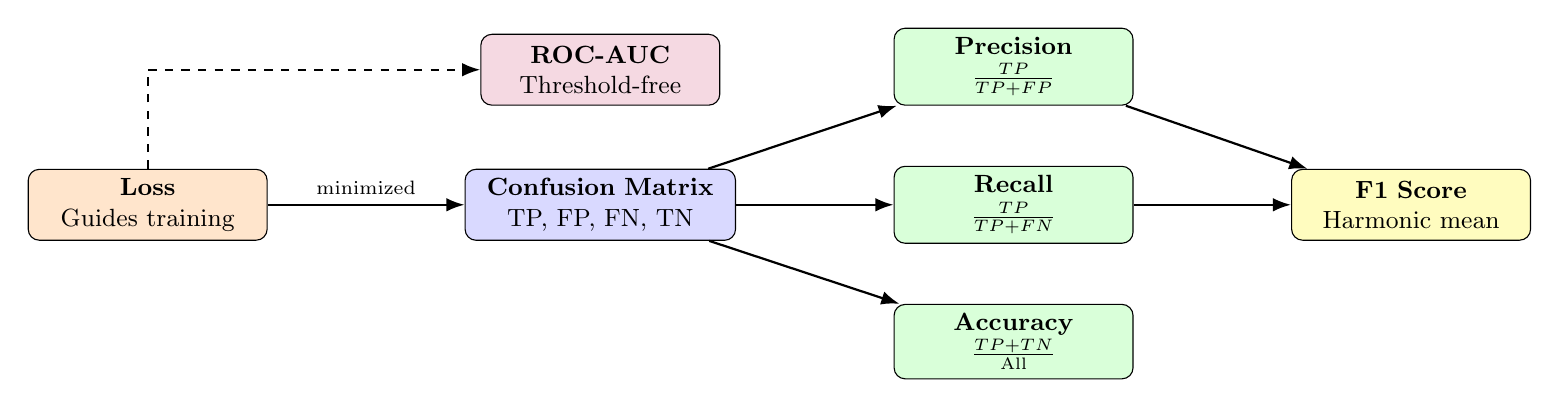
\begin{tikzpicture}[
    node distance=1cm and 1.5cm,
    box/.style={draw, rectangle, rounded corners, align=center, text width=2.8cm, minimum height=0.9cm, font=\small},
    arrow/.style={-Latex, thick},
]
    % Training side
    \node[box, fill=orange!20] (loss) {\textbf{Loss}\\Guides training};

    % Confusion matrix at center
    \node[box, fill=blue!15, right=2.5cm of loss, text width=3.2cm] (cm) {\textbf{Confusion Matrix}\\TP, FP, FN, TN};

    % Derived metrics
    \node[box, fill=green!15, above right=0.8cm and 2cm of cm] (prec) {\textbf{Precision}\\$\frac{TP}{TP+FP}$};
    \node[box, fill=green!15, right=2cm of cm] (rec) {\textbf{Recall}\\$\frac{TP}{TP+FN}$};
    \node[box, fill=green!15, below right=0.8cm and 2cm of cm] (acc) {\textbf{Accuracy}\\$\frac{TP+TN}{\text{All}}$};

    % F1 from Precision and Recall
    \node[box, fill=yellow!25, right=2cm of rec] (f1) {\textbf{F1 Score}\\Harmonic mean};

    % ROC separate
    \node[box, fill=purple!15, above=0.8cm of cm] (roc) {\textbf{ROC-AUC}\\Threshold-free};

    % Arrows
    \draw[arrow] (loss) -- node[above, font=\scriptsize] {minimized} (cm);
    \draw[arrow] (cm) -- (prec);
    \draw[arrow] (cm) -- (rec);
    \draw[arrow] (cm) -- (acc);
    \draw[arrow] (prec) -- (f1);
    \draw[arrow] (rec) -- (f1);
    \draw[arrow, dashed] (loss.north) |- (roc.west);

\end{tikzpicture}
\end{center}

\noindent \textbf{Reading the diagram:}
\begin{itemize}[noitemsep]
    \item \textbf{Loss} drives training and indirectly determines how well the model separates classes.
    \item After training, predictions are summarized in the \textbf{Confusion Matrix}.
    \item From the confusion matrix, we derive \textbf{Precision}, \textbf{Recall}, and \textbf{Accuracy}.
    \item \textbf{F1 Score} combines Precision and Recall into a single balanced number.
    \item \textbf{ROC-AUC} is computed from the raw probabilities (before thresholding) and tells us the model's separability power.
\end{itemize}

% ============================================================================
\section{Quick Reference: When to Use Which Metric}
% ============================================================================

\begin{center}
\renewcommand{\arraystretch}{1.3}
\begin{tabularx}{\textwidth}{@{}lX@{}}
\toprule
\textbf{Situation} & \textbf{Primary Metric} \\
\midrule
Quick overall check                    & Accuracy \\
Safety-critical (must not miss events) & \textbf{Recall} \\
Resource-limited (false alarms costly) & Precision \\
Balanced comparison between models     & F1 Score \\
Comparing models before choosing threshold & ROC-AUC \\
Debugging which classes are problematic & Confusion Matrix \\
Monitoring if training is progressing  & Loss \\
\bottomrule
\end{tabularx}
\end{center}

\end{document}
